\documentclass[10pt]{article}
\usepackage[utf8]{inputenc}
\usepackage[T1]{fontenc}
\usepackage{amsmath}
\usepackage{amsfonts}
\usepackage{amssymb}
\usepackage[version=4]{mhchem}
\usepackage{stmaryrd}
\usepackage{graphicx}
\usepackage[export]{adjustbox}
\graphicspath{ {./images/} }

\title{EXTRA MATHEMATICS ADMISSIONS TEST December 2021 \\
 Time allowed: 1 hour }

\author{}
\date{}


\begin{document}
\maketitle
\begin{center}
\begin{tabular}{|l|l|}
\hline
Surname &  \\
\hline
Other names &  \\
\hline
\end{tabular}
\end{center}

This paper contains 10 multiple choice questions.

\section*{Calculators are not permitted.}
For each question on pages 2-11 you will be given five possible answers, just one of which is correct. Indicate for each question $\mathbf{A}-\mathbf{J}$ which answer (a), (b), (c), (d), or (e) you think is correct with a tick $(\checkmark)$ in the corresponding column in the table below.

\begin{center}
\begin{tabular}{|c|l|l|l|l|l|}
\hline
 & $(\mathrm{a})$ & $(\mathrm{b})$ & $(\mathrm{c})$ & $(\mathrm{d})$ & $(\mathrm{e})$ \\
\hline
A &  &  &  &  &  \\
\hline
B &  &  &  &  &  \\
\hline
C &  &  &  &  &  \\
\hline
D &  &  &  &  &  \\
\hline
E &  &  &  &  &  \\
\hline
F &  &  &  &  &  \\
\hline
G &  &  &  &  &  \\
\hline
H &  &  &  &  &  \\
\hline
I &  &  &  &  &  \\
\hline
\end{tabular}
\end{center}

A. Which of the following expressions has the largest value? Note that all angles are given in degrees.

(a) $\cos \left(10^{\circ}\right)$,

(b) $\sin \left(115^{\circ}\right)$,

(c) $\cos \left(375^{\circ}\right)$,

(d) $\sin \left(85^{\circ}\right)$,

(e) $\cos \left(-20^{\circ}\right)$.

B. In the expansion of $\left(x^{2}+x y+y^{2}\right)^{n}$, where $n$ is a positive whole number, the coefficient of $x^{3} y^{2 n-3}$ is

(a) $\left(\begin{array}{l}n \\ 3\end{array}\right)$

(b) $\left(\begin{array}{l}n \\ 3\end{array}\right) \times\left(\begin{array}{l}n \\ 2\end{array}\right)$

(c) $\left(\begin{array}{l}n \\ 3\end{array}\right)+2 \times\left(\begin{array}{l}n \\ 2\end{array}\right)$

(d) $2 \times\left(\begin{array}{l}n \\ 2\end{array}\right)$

(e) $\left(\begin{array}{l}n \\ 3\end{array}\right)+\left(\begin{array}{l}n \\ 2\end{array}\right)$

C. Given a real number $c$ with $0<c<1$, the line $y=c$ intersects the circle $x^{2}+y^{2}=1$ at two points. These two points, together with $(1,0)$ and $(-1,0)$, form a quadrilateral. Which of the following graphs is a plot of the area of that quadrilateral against $c$ ?

(a)

\begin{center}
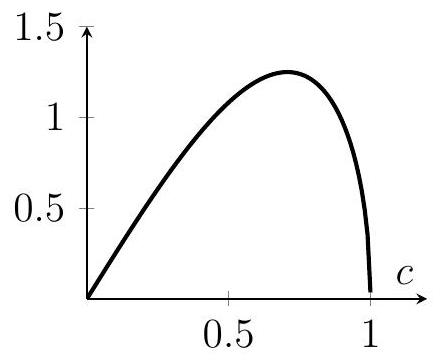
\includegraphics[max width=\textwidth]{2024_03_31_c94a599a3f94f0a66112g-04(1)}
\end{center}

(b)

\begin{center}
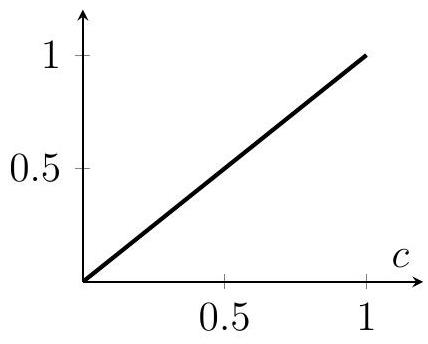
\includegraphics[max width=\textwidth]{2024_03_31_c94a599a3f94f0a66112g-04}
\end{center}

(c)

\begin{center}
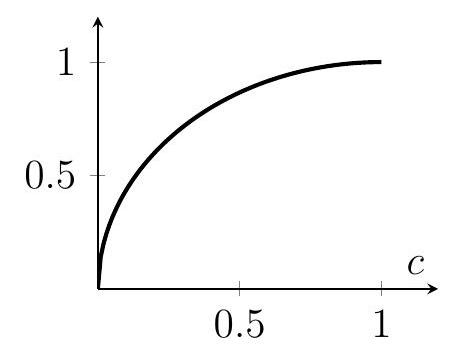
\includegraphics[max width=\textwidth]{2024_03_31_c94a599a3f94f0a66112g-04(4)}
\end{center}

(d)

\begin{center}
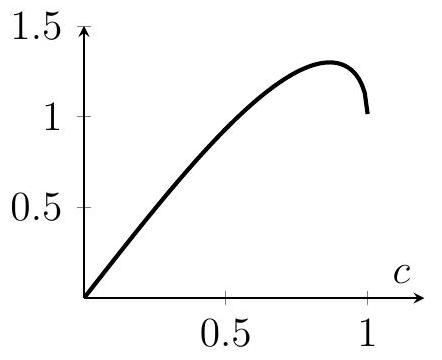
\includegraphics[max width=\textwidth]{2024_03_31_c94a599a3f94f0a66112g-04(3)}
\end{center}

(e)

\begin{center}
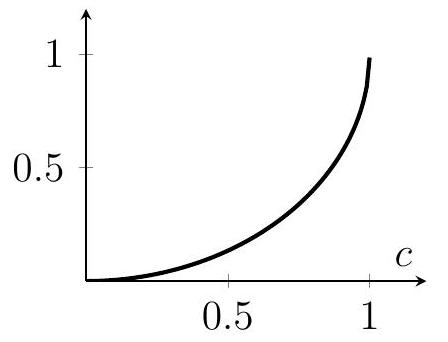
\includegraphics[max width=\textwidth]{2024_03_31_c94a599a3f94f0a66112g-04(2)}
\end{center}

D. A particle moves along the $x$-axis. At time $t=0$ the particle starts at $(0,0)$ with initial speed 1 , moving towards $x=1$. When the particle reaches $x=n$ for any positive integer $n$, its speed immediately changes to $2^{-n}$ but its direction is unchanged. What is the particle's position at time $t=100$ ?

(a) $x=\frac{89}{16}$,

(b) $x=\frac{105}{16}$,

(c) $x=\frac{3200}{32}$,

(d) $x=\frac{421}{64}$,

(e) The particle has escaped to infinity.

E. The polynomial equation $x^{4}-(2 k+1) x^{2}+2 x+k^{2}-1=0$ has exactly four real solutions $x$ if and only if

(a) $k>1$,

(b) $k>-\frac{5}{4}$,

(c) $k>\frac{3}{4}$,

(d) $k<-\frac{5}{4}$ or $k>\frac{3}{4}$,

(e) $\frac{3}{4}<k<1$ or $k>1$.

F. The point $A$ has coordinates $(3,4)$. The origin $(0,0)$ and the point $A$ both lie on the circumference of a circle $\mathcal{C}$. The diameter of $\mathcal{C}$ through $A$ also meets $\mathcal{C}$ at another point $B$. The distance between $B$ and the origin is 10 . It follows that the coordinates of $B$ could be either

(a) $(-5 \sqrt{2}, 5 \sqrt{2})$ or $(5 \sqrt{2},-5 \sqrt{2})$,

(b) $(-4,3)$ or $(4,-3)$,

(c) $(-5,5 \sqrt{3})$ or $(5,-5 \sqrt{3})$,

(d) $(-8,6)$ or $(8,-6)$,

(e) $(-5 \sqrt{3}, 5)$ or $(5 \sqrt{3},-5)$.

G. Without calculating it directly, which of the following numbers is the square of $123,456,789$ ?

(a) $15,241,578,710,190,521$,

(b) $15,241,578,730,190,521$,

(c) $15,241,578,750,190,521$,

(d) $15,241,578,770,190,521$,

(e) $15,241,578,790,190,521$.

H. A function $f(x)$ satisfies the following equation

$$
f(x)+f(y)=\frac{1}{f(x y)}
$$

for any real positive numbers $x$ and $y$, and also satisfies $f(x)>0$ for all real positive numbers $x$. It follows that $f(2021)$ is

(a) 1 ,

(b) 2021,

(c) $\log _{e} 2021$,

(d) $\frac{1}{\sqrt{2}}$,

(e) $\frac{1}{\log _{e} 2021}$.

[Hint: try substituting $x=1$ and $y=1$ into the given expression.]

I. Given that there are positive real numbers $a, b, c$ that satisfy

$$
\int_{a}^{b} \log _{c}\left(\sin ^{4} x \tan ^{2} x\right) \mathrm{d} x=1 \text { and } \int_{a}^{b} \log _{c}\left(\sin ^{2} x \cos ^{2} x\right) \mathrm{d} x=3
$$

it follows that the value of

$$
\int_{a}^{b} \log _{c}\left(\sin ^{4} x \cos ^{2} x\right) \mathrm{d} x
$$

must be equal to

(a) 4 ,

(b) 5 ,

(c) 6 ,

(d) 7 ,

(e) 8 .

$\left[\right.$ Note that $\sin ^{4} x$ means $(\sin x)^{4}$.]

J. There is a straight line that is normal to the curve $y=x^{3}-k x$ at two different points if and only if

(a) $k \geq \sqrt{3}$,

(b) $k^{2} \geq 3$,

(c) $k^{2} \geq 1$,

(d) $k \geq 1$,

(e) $k \geq \sqrt{3}$ or $k \leq-1$.


\end{document}